\documentclass[tikz,border=2mm]{standalone}
\usepackage{tikz}
\usetikzlibrary{matrix,arrows.meta,positioning,calc}

\tikzset{
    level0/.style={rectangle, draw=black, fill=magenta!30, font=\bfseries\large, minimum width=2cm, minimum height=1cm},
    level1/.style={rectangle, draw=black, fill=green!50!white, font=\bfseries\large, minimum width=2cm, minimum height=1cm},
    level2/.style={rectangle, draw=black, fill=blue!40!white, font=\bfseries\large, minimum width=2cm, minimum height=1cm},
    level3/.style={rectangle, draw=black, fill=orange!40!white, font=\bfseries\large, minimum width=2cm, minimum height=1cm},
    newOp/.style={line width=2pt},
    transparent/.style={opacity=0.3},
    dashed/.style={dash pattern=on 4pt off 2pt, opacity=0.9}
}

\begin{document}
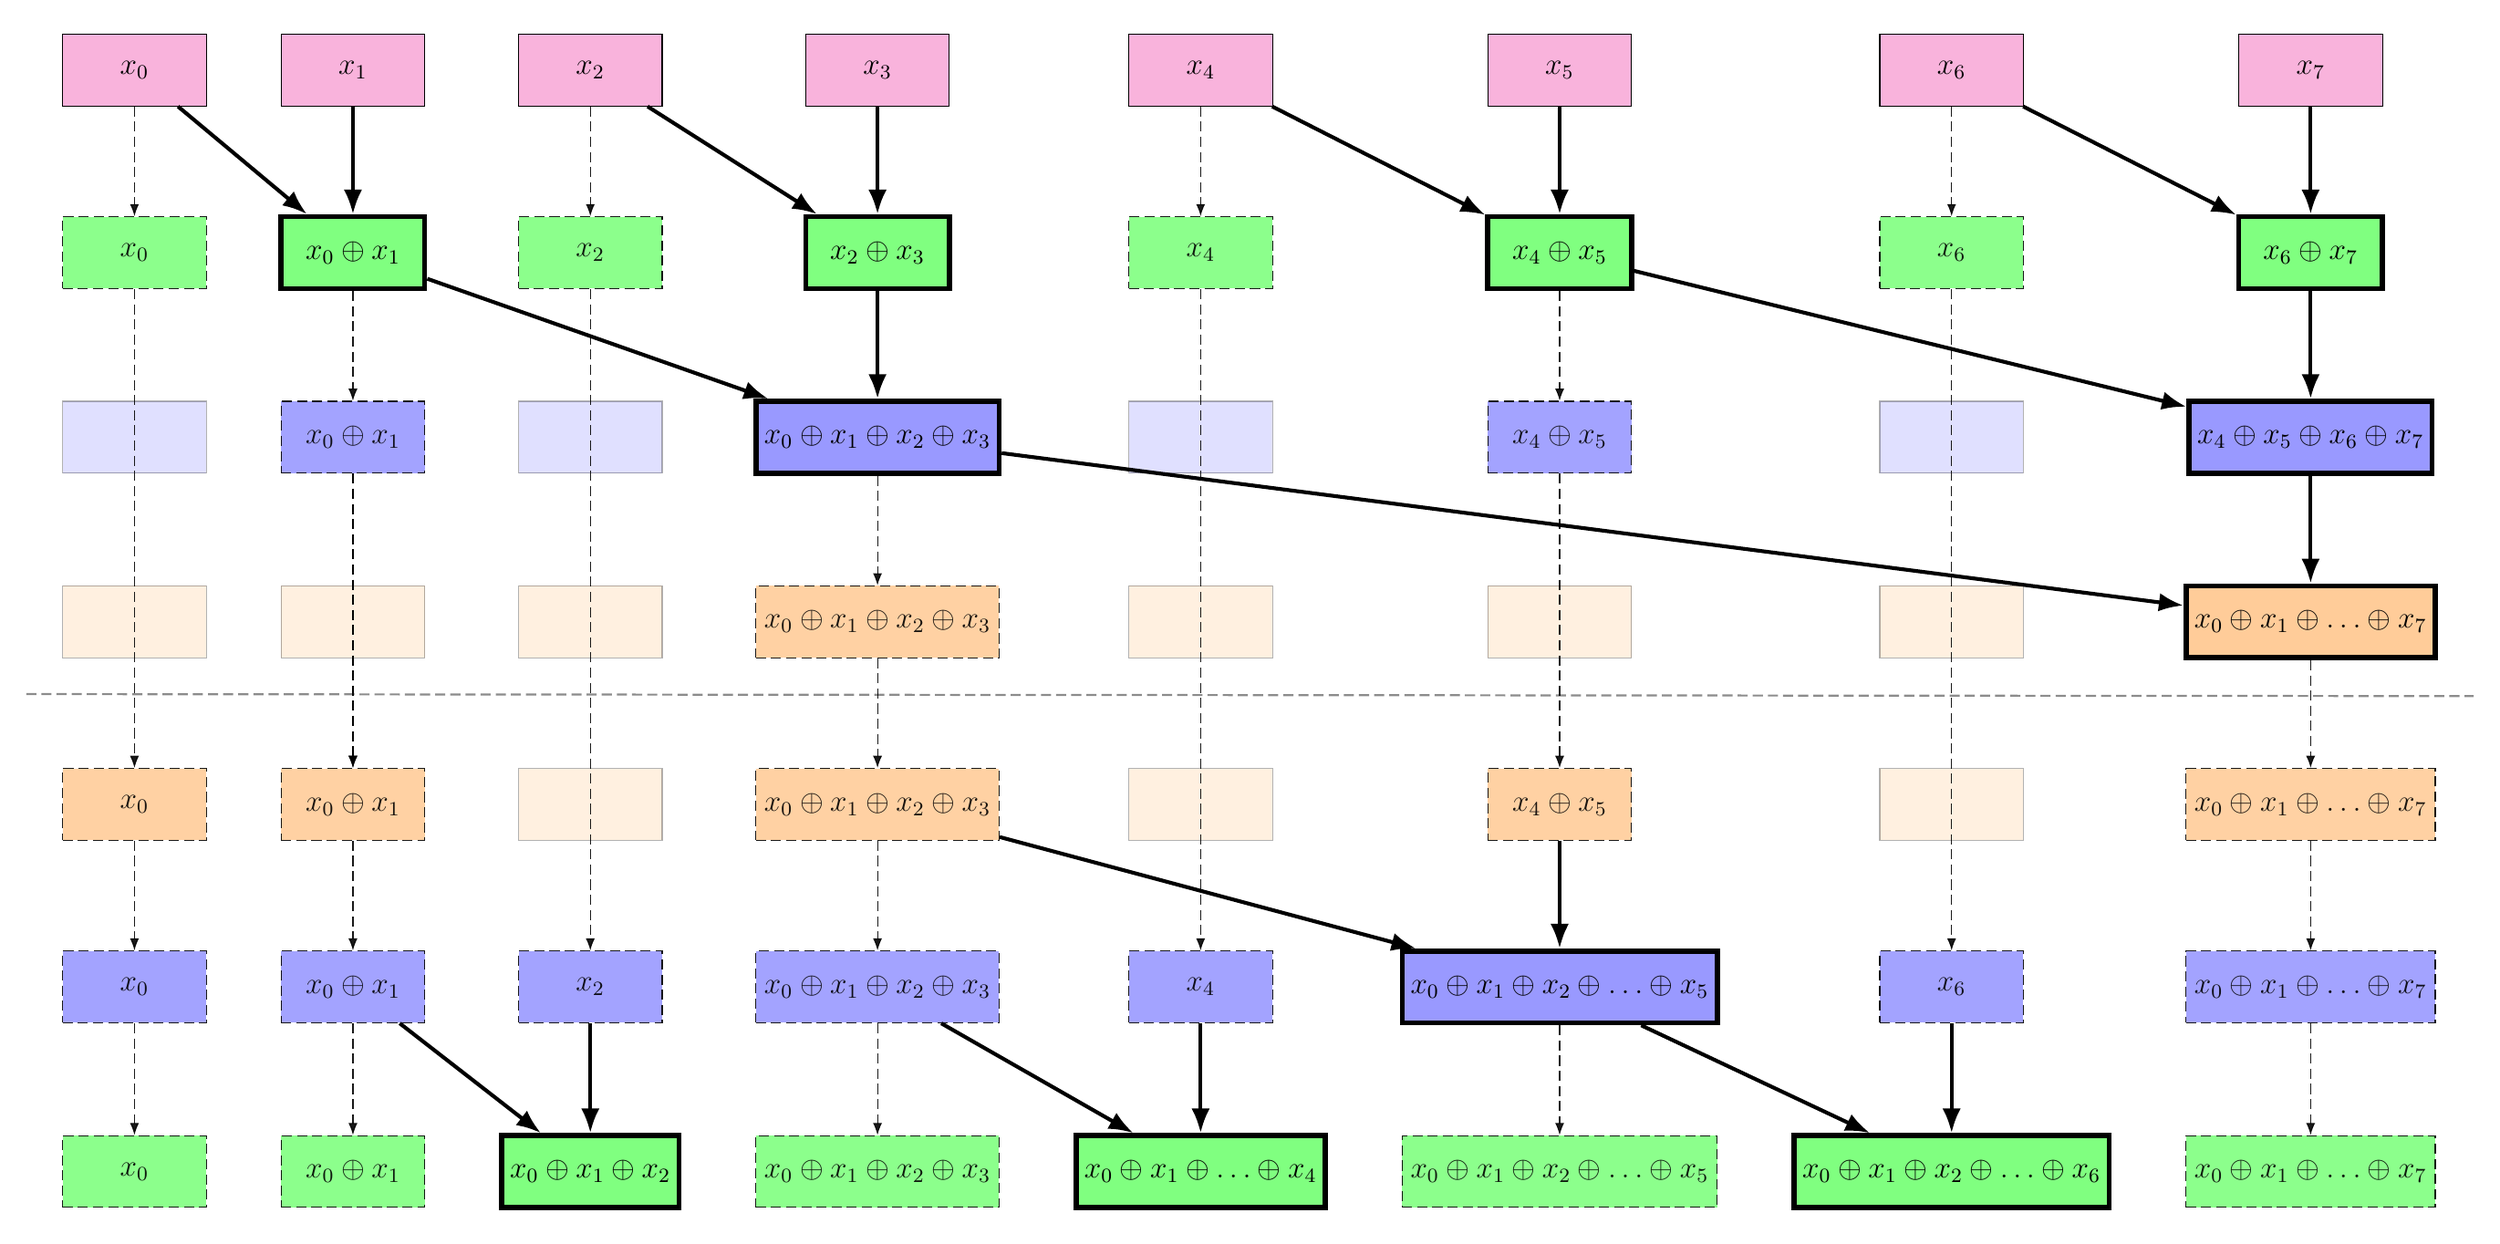
\begin{tikzpicture}[>=Latex]

\matrix[column sep=1cm, row sep=1.5cm] (m) {
  % Row 0: leaves
  \node[level0] (x0) {$x_0$}; & \node[level0] (x1) {$x_1$}; & \node[level0] (x2) {$x_2$}; & \node[level0] (x3) {$x_3$}; &
  \node[level0] (x4) {$x_4$}; & \node[level0] (x5) {$x_5$}; & \node[level0] (x6) {$x_6$}; & \node[level0] (x7) {$x_7$}; \\
  
  % Row 1: Level 1
  \node[level1,dashed] (y0) {$x_0$}; & \node[level1,newOp] (y1) {$x_0 \oplus x_1$}; &
  \node[level1,dashed] (y2) {$x_2$}; & \node[level1,newOp] (y3) {$x_2 \oplus x_3$}; &
  \node[level1,dashed] (y4) {$x_4$}; & \node[level1,newOp] (y5) {$x_4 \oplus x_5$}; &
  \node[level1,dashed] (y6) {$x_6$}; & \node[level1,newOp] (y7) {$x_6 \oplus x_7$}; \\
  
  % Row 2: Level 2
  \node[level2,transparent] (z0) {~}; & \node[level2,dashed] (z1) {$x_0 \oplus x_1$}; &
  \node[level2,transparent] (z2) {~}; & \node[level2,newOp] (z3) {$x_0 \oplus x_1 \oplus x_2 \oplus x_3$}; &
  \node[level2,transparent] (z4) {~}; & \node[level2,dashed] (z5) {$x_4 \oplus x_5$}; &
  \node[level2,transparent] (z6) {~}; & \node[level2,newOp] (z7) {$x_4 \oplus x_5 \oplus x_6 \oplus x_7$}; \\
  
  % Row 3: Level 3
  \node[level3,transparent] (w0) {~}; & \node[level3,transparent] (w1) {~}; & \node[level3,transparent] (w2) {~}; &
  \node[level3,dashed] (w3) {$x_0 \oplus x_1 \oplus x_2 \oplus x_3$}; &
  \node[level3,transparent] (w4) {~}; & \node[level3,transparent] (w5) {~}; & \node[level3,transparent] (w6) {~}; &
  \node[level3,newOp] (w7) {$x_0 \oplus x_1 \oplus \dots \oplus x_7$}; \\
  
  % Row 4: down-sweep (transparent placeholders)
  \node[level3,dashed] (d0) {$x_0$}; & \node[level3,dashed] (d1) {$x_0 \oplus x_1$}; & \node[level3,transparent] (d2) {~}; &
  \node[level3,dashed] (d3) {$x_0 \oplus x_1 \oplus x_2 \oplus x_3$}; & \node[level3,transparent] (d4) {~}; & \node[level3,dashed] (d5) {$x_4 \oplus x_5$}; &
  \node[level3,transparent] (d6) {~}; & \node[level3,dashed] (d7) {$x_0 \oplus x_1 \oplus \dots \oplus x_7$}; \\
  
  % Row 5: down-sweep intermediate
  \node[level2,dashed] (e0) {$x_0$}; & \node[level2,dashed] (e1) {$x_0 \oplus x_1$}; & \node[level2,dashed] (e2) {$x_2$}; &
  \node[level2,dashed] (e3) {$x_0 \oplus x_1 \oplus x_2 \oplus x_3$}; & \node[level2,dashed] (e4) {$x_4$}; & \node[level2,newOp] (e5) {$x_0 \oplus x_1 \oplus x_2 \oplus \dots \oplus x_5$}; &
  \node[level2,dashed] (e6) {$x_6$}; & \node[level2,dashed] (e7) {$x_0 \oplus x_1 \oplus \dots \oplus x_7$}; \\
  
  % Row 6: down-sweep
  \node[level1,dashed] (f0) {$x_0$}; & \node[level1,dashed] (f1) {$x_0 \oplus x_1$}; & \node[level1,newOp] (f2) {$x_0 \oplus x_1 \oplus x_2$}; &
  \node[level1,dashed] (f3) {$x_0 \oplus x_1 \oplus x_2 \oplus x_3$}; & \node[level1,newOp] (f4) {$x_0 \oplus x_1 \oplus \dots \oplus x_4$}; & \node[level1,dashed] (f5) {$x_0 \oplus x_1 \oplus x_2 \oplus \dots \oplus x_5$}; &
  \node[level1,newOp] (f6) {$x_0 \oplus x_1 \oplus x_2 \oplus \dots \oplus x_6$}; & \node[level1,dashed] (f7) {$x_0 \oplus x_1 \oplus \dots \oplus x_7$}; \\
};

% ----------------------------
% Up-sweep arrows
% ----------------------------
\foreach \i/\j in {0/1,2/3,4/5,6/7} {
  \draw[->,line width=1.5pt] (x\i) -- (y\j);
  \draw[->,line width=1.5pt] (x\j) -- (y\j);
}
\draw[->,line width=1.5pt] (y1) -- (z3);
\draw[->,line width=1.5pt] (y3) -- (z3);
\draw[->,line width=1.5pt] (y5) -- (z7);
\draw[->,line width=1.5pt] (y7) -- (z7);
\draw[->,line width=1.5pt] (z3) -- (w7);
\draw[->,line width=1.5pt] (z7) -- (w7);

\draw[->, dashed] (x0) -- (y0);
\draw[->, dashed] (x2) -- (y2);
\draw[->, dashed] (x4) -- (y4);
\draw[->, dashed] (x6) -- (y6);
\draw[->, dashed] (y1) -- (z1);
\draw[->, dashed] (y5) -- (z5);
\draw[->, dashed] (z3) -- (w3);

\draw[->, dashed] (y6) -- (e6);
\draw[->, line width=1.5pt] (e6) -- (f6);
\draw[->, line width=1.5pt] (e5) -- (f6);

\draw[->, dashed] (z1) -- (d1);

% ----------------------------
% Separator line
% ----------------------------
\draw[thick, gray, dashed] ($(w0.south west)+(-0.5,-0.5)$) -- ($(w7.south east)+(0.5,-0.5)$);

% ----------------------------
% Down-sweep arrows (stopping at f row)
% ----------------------------
\draw[->, dashed] (w7) -- (d7);
\draw[->, dashed] (d7) -- (e7);
\draw[->, dashed] (e7) -- (f7);

\draw[->,dashed] (y0) -- (d0);
\draw[->,dashed] (d0) -- (e0);
\draw[->,dashed] (e0) -- (f0);

\draw[->,dashed] (w3) -- (d3);
\draw[->,dashed] (d3) -- (e3);
\draw[->,dashed] (e3) -- (f3);

\draw[->,dashed] (z5) -- (d5);
\draw[->,line width=1.5pt] (d5) -- (e5);
\draw[->,line width=1.5pt] (d3) -- (e5);
\draw[->,dashed] (e5) -- (f5);

\draw[->,dashed] (y4) -- (e4);
\draw[->,line width=1.5pt] (e4) -- (f4);
\draw[->,line width=1.5pt] (e3) -- (f4);

\draw[->,dashed] (z1) -- (d1);
\draw[->,dashed] (d1) -- (e1);
\draw[->,dashed] (e1) -- (f1);

\draw[->,dashed] (y2) -- (e2);
\draw[->,line width=1.5pt] (e2) -- (f2);
\draw[->,line width=1.5pt] (e1) -- (f2);

\end{tikzpicture}
\end{document}
